\chapter{Reference Simulator}
\label{ch:refsim}

\Cref{ch:problem} laid out the prediction and control problem and the tensor format used to represent a train.
This chapter builds the tool that actually produces the numbers: a reference simulator of longitudinal train dynamics.
Its job is simple to state even though the physics inside it is not.
Given a train made of coupled vehicles, a route, and a set of driving commands, the simulator plays out what happens over time and records it.
Every training example used later to teach the surrogate model comes from running this simulator once, so in that sense this chapter describes the data generator for the rest of the thesis.

The simulator was built up gradually, one physical effect at a time, so that each addition could be checked before the next was layered on.
It follows a Jupyter notebook that constructs the model stage by stage using only NumPy, SciPy's \texttt{solve\_ivp}, and Matplotlib, and the same model is mirrored in a structured Python package that exposes the node and edge tensors from \cref{ch:problem} alongside the classical flat state used for integration.

The parameters used, vehicle mass, resistance coefficients, coupler stiffness, traction limits, are realistic in shape but are not tuned to match any specific real locomotive or railcar.
The goal at this stage is a simulator whose structure is right, not one whose numbers are certified against a real test train.
This distinction matters when interpreting later results: the surrogate and the control experiments built on top of this simulator are validated against the simulator itself, not against real-world rail data.
Time integration uses adaptive Runge-Kutta or implicit methods as needed when stiff coupler dynamics appear, and the figures in this chapter are exported directly from the notebook at representative numerical settings.

\section{Stage 1: single powered vehicle}

The starting point is a single point mass $m$ with longitudinal position $x(t)$ and velocity $v(t)=\dot{x}$. The equation of motion aggregates traction, braking, Davis running resistance, grade, and an optional curve resistance into a single scalar force balance:
\begin{equation}
    m\dot{v} = F_{\mathrm{trac}}(t) - F_{\mathrm{brk}}(t) - R(v) - G(x) - C_{\kappa}(x,v),
    \label{eq:ltd_stage1}
\end{equation}
with $\dot{x}=v$. Davis resistance is implemented in the usual magnitude-direction form,
\begin{equation}
    R(v) = \bigl(A + B|v| + C v^2\bigr)\,\mathrm{sgn}(v),
    \label{eq:ltd_davis}
\end{equation}
with $\mathrm{sgn}(v)$ set to zero at $|v|<\varepsilon$ to avoid chatter at standstill. Note that the coefficient $C$ in \cref{eq:ltd_davis} is the Davis quadratic term and is unrelated to the curve resistance $C_{\kappa}$. Grade enters through $G(x)=mg\sin\theta(x)$ with $\theta$ the local track inclination.

Curve resistance is written, as is standard in railway practice, as a \emph{specific} resistance $w_c$: a fraction of vehicle weight fixed by the curve radius $R=1/|\kappa|$ and independent of speed. The implementation uses the linear (AREMA) form,
\begin{equation}
    C_{\kappa}(x,v) = c_{\kappa}\, m g\, w_c\bigl(\kappa(x)\bigr)\,\mathrm{sgn}(v),
    \qquad
    w_c(\kappa) = \lambda\,|\kappa|,
    \label{eq:ltd_curvature}
\end{equation}
with $\lambda \approx 0.699$, the AREMA figure of 0.8 lb per ton per degree of curve expressed in terms of $\kappa$, and $c_{\kappa}$ a dimensionless multiplier for which $c_{\kappa}=1$ recovers the standard value. The term is disabled by setting $c_{\kappa}=0$, which is the case in the earliest runs and in any scenario that does not require it. On the corridors used here the force is small but not negligible: at the 95th-percentile curvature (radius $\approx$ 840 m) it is roughly 800 N on a loaded 100 t car, comparable to that car's Davis resistance at 15 m/s and about 8\% of the force of a 1\% grade.

Two aspects of \cref{eq:ltd_curvature} are stated explicitly because both were settled by measurement rather than by convention. The first is the absence of a speed dependence. Earlier revisions used a proxy proportional to $m v^{2}|\kappa(x)|$; that form is retained in the implementation so results recorded before this change can be reproduced, but it is not the model of record. Curve resistance does not scale with speed, so a coefficient matched to \cref{eq:ltd_curvature} at one speed is wrong at every other --- one calibrated at 15 m/s is nine times too small at 5 m/s and 2.8 times too large at 25 m/s. The discrepancy is in the exponent rather than the constant, so no choice of scale repairs it. The second is the choice of $w_c$. The R\"ockl formula, $w_c = 650/(R-55)$ N/kN for $R \geq 300$ m and $500/(R-30)$ below, is the more familiar empirical statement and agrees with \cref{eq:ltd_curvature} to within about 15\% over the 300--2000 m range these routes occupy. It is available in the implementation but is not the default, because it is discontinuous at $R = 300$ m, where its two branches differ by roughly 30\%. This force balance is the generator of the training data, so a jump in it becomes a jump in the trajectories the surrogate learns from, one the learned fixed step would have to reproduce whenever a vehicle crosses $R = 300$\,m within a step. The controller, in turn, takes its gradients from the surrogate rather than from this force balance, so it is the surrogate's behaviour near such a jump that the controller would see. The reasoning is the same as that behind the $\tanh$ blend in \cref{eq:ltd_brake_sign}. The distinction being drawn is between a jump and a kink: piecewise-linear interpolation of the route field already makes $\partial C_{\kappa}/\partial x$ discontinuous at every route node, and the coupler deadband of Stage~3 does the same at slack transitions, but in both cases the force itself remains continuous. R\"ockl would instead make the force discontinuous, which is a stronger defect and, unlike the other two, one the model does not need.

Traction and brake commands may be specified as arbitrary functions of time; the first stage uses a smooth ``ramp'' in time so that $F_{\mathrm{trac}}$ rises continuously from zero after a delay, rather than stepping instantaneously, which eases numerical stiffness and mirrors the later actuator-lag extension. \Cref{fig:ltd_stage01} shows position, speed, and the plotted residual $F_{\mathrm{trac}}-R(v)$ on level track with braking and curvature removed, confirming that the integrator and force signs behave as intended before couplers are introduced.

\begin{figure}[htbp]
    \centering
    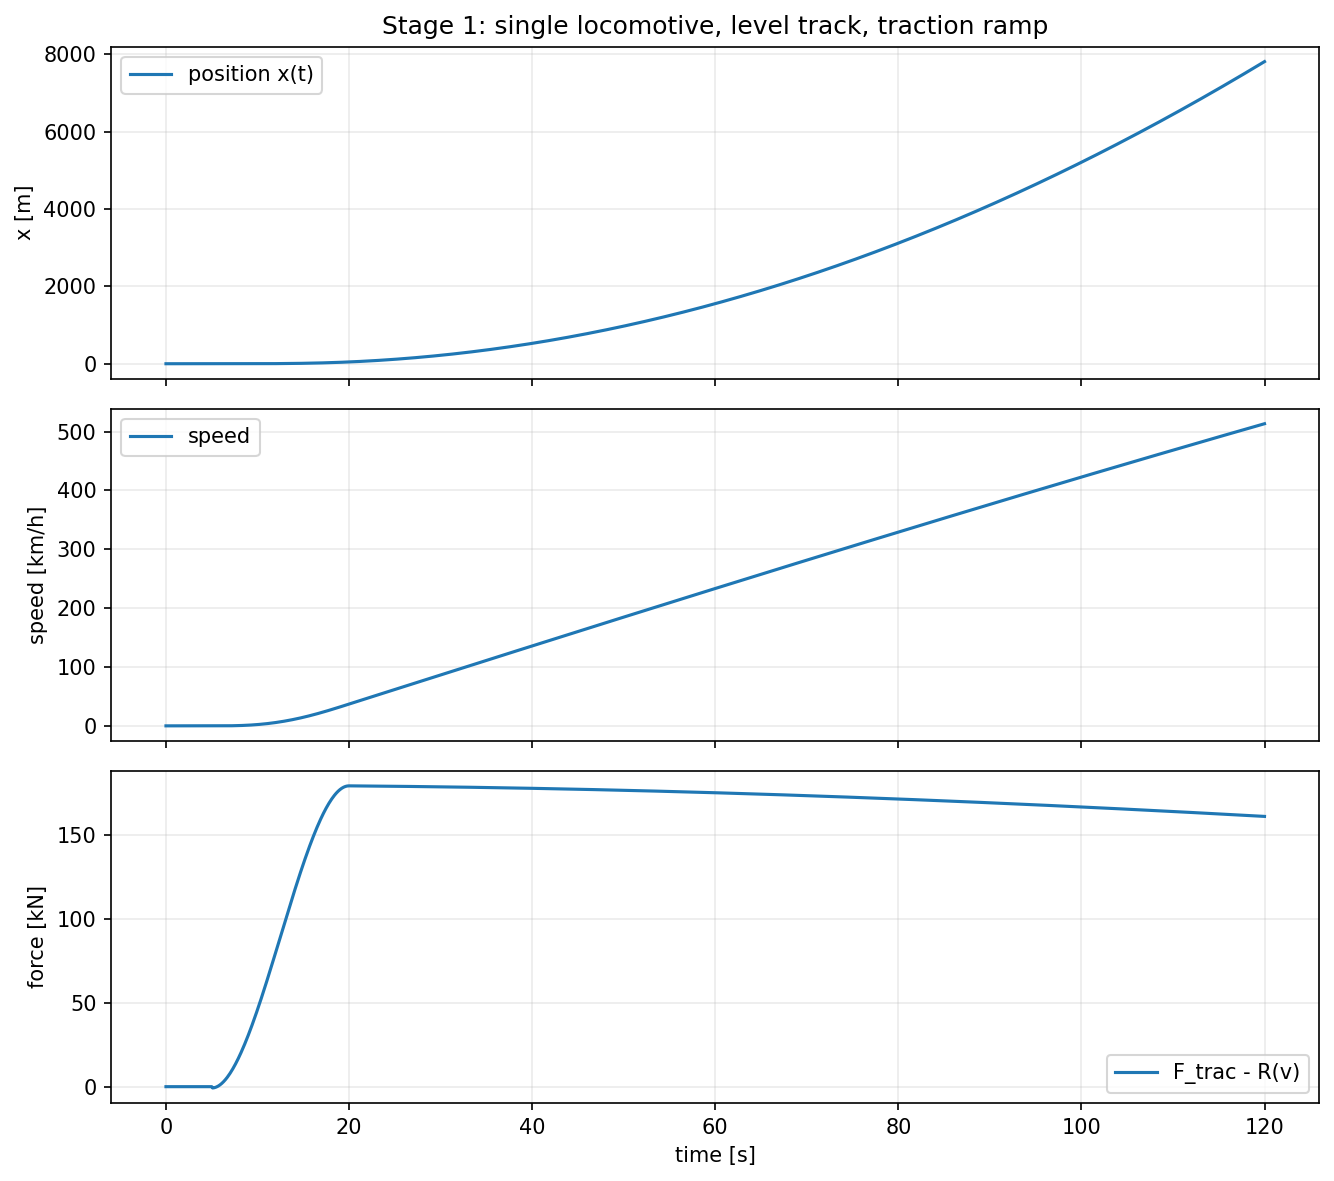
\includegraphics[width=0.92\textwidth]{../notebooks/notebook_images/ltd_stage01_single_loco_traction_ramp_position_speed_netforce.png}
    \caption{Stage~1 reference run: single vehicle on level track with a smooth traction ramp. Top to bottom: position, speed, and net longitudinal force $F_{\mathrm{trac}}-R(v)$ versus time.}
    \label{fig:ltd_stage01}
\end{figure}

\section{Stage 2: locomotive and one car with a linear coupler}

A second mass $m_1$ is attached behind the lead vehicle $m_0$. Nominal centre-to-centre spacing is $L_0$. Coupler extension (positive in draft) is
\begin{equation}
    \delta = (x_0 - x_1) - L_0, \qquad \dot{\delta} = v_0 - v_1.
    \label{eq:ltd_delta}
\end{equation}
A linear spring-damper coupler exerts force $F = k\delta + c\dot{\delta}$ on the rear car along the direction of travel; the lead feels $-F$. With $G_i$ and $R_i$ evaluated per vehicle,
\begin{align}
    m_0 \dot{v}_0 &= F_{\mathrm{trac}} - F_{\mathrm{brk},0} - R_0(v_0) - G_0(x_0) - F, \\
    m_1 \dot{v}_1 &= -F_{\mathrm{brk},1} - R_1(v_1) - G_1(x_1) + F.
    \label{eq:ltd_stage2}
\end{align}
The state vector is $(x_0,x_1,v_0,v_1)$. For stiff $(k,c)$ the two speeds track almost identically on a speed-time plot even though the coupler force and extension carry the load path; \cref{fig:ltd_stage02} shows the characteristic transient in $F$ and $\delta$ as slack is taken up and the train settles into quasi-uniform acceleration under traction.

\begin{figure}[htbp]
    \centering
    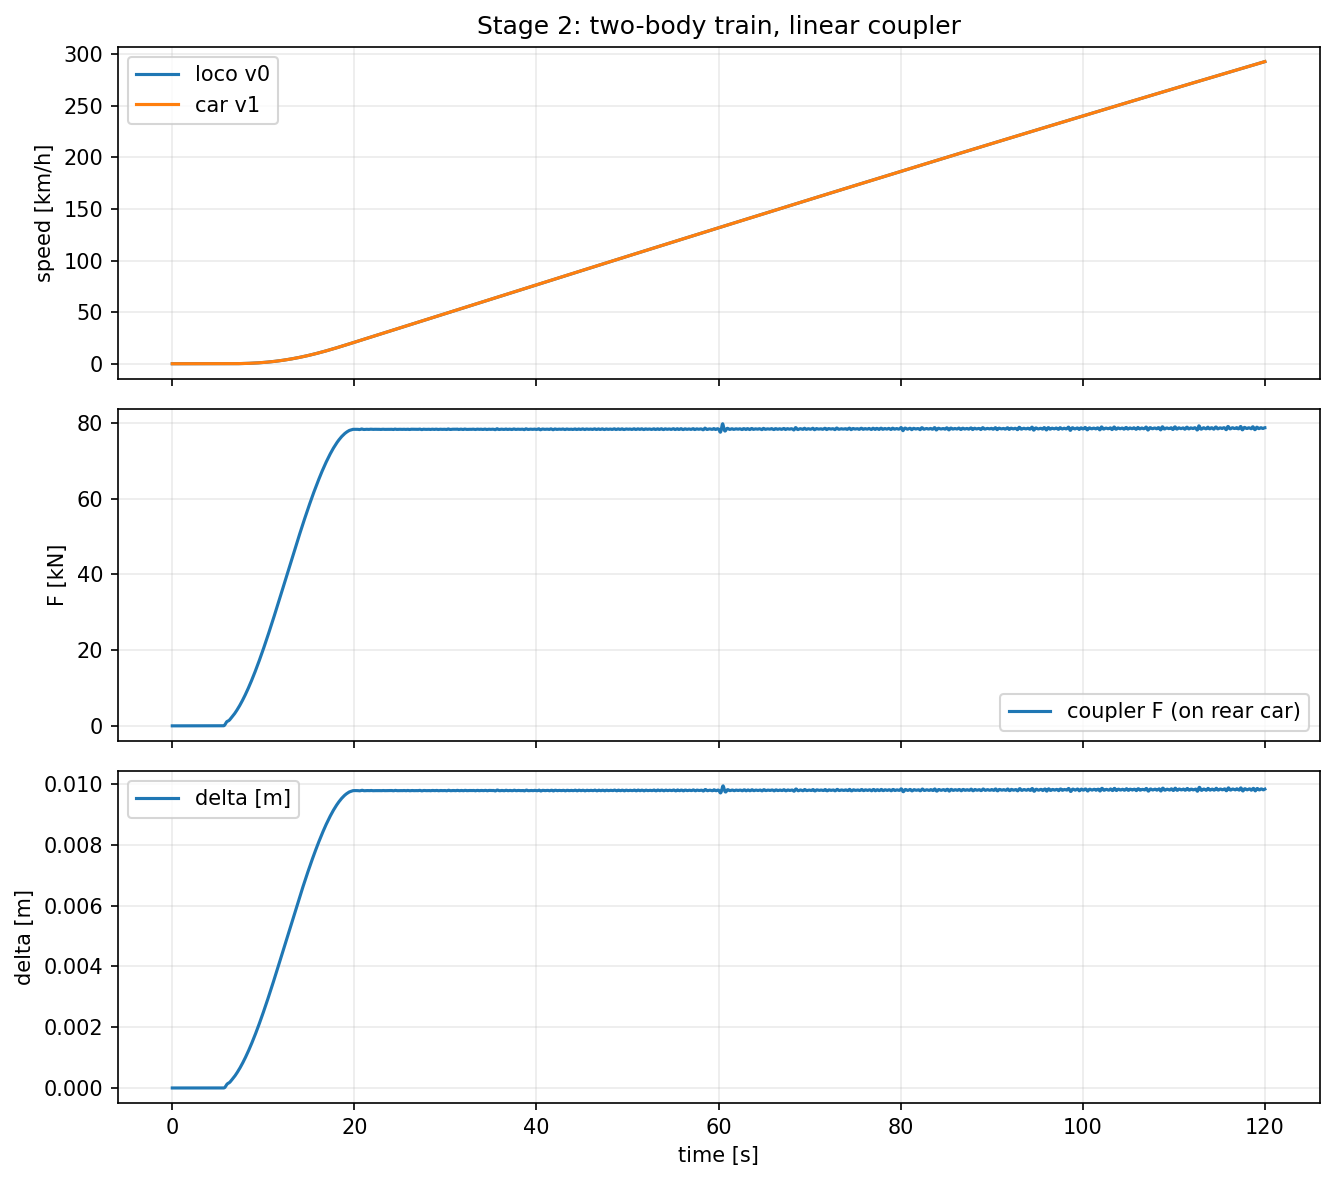
\includegraphics[width=0.92\textwidth]{../notebooks/notebook_images/ltd_stage02_loco_car_speeds_coupler_force_extension.png}
    \caption{Stage~2: two-body train with linear coupler. Speeds of lead and trailing vehicle (overlapping at this scale), coupler force on the rear car, and extension $\delta$.}
    \label{fig:ltd_stage02}
\end{figure}

\section{Stage 3: nonlinear coupler with slack and asymmetric buff/draft}

The linear model is retained for comparison, but the simulated dynamics replace $F$ by a piecewise law with slack half-width $s$. For $|\delta|\le s$ the coupler force is zero; for $\delta>s$ (draft) stiffness and damping $(k_{\mathrm{d}},c_{\mathrm{d}})$ apply to the over-travel $\delta-s$, and for $\delta<-s$ (buff) a possibly different pair $(k_{\mathrm{b}},c_{\mathrm{b}})$ applies to $\delta+s$. The same two-body equations \cref{eq:ltd_stage2} hold with this $F(\delta,\dot{\delta})$. \Cref{fig:ltd_stage03} overlays the \emph{linear} force $k\delta+c\dot{\delta}$ that would correspond to Stage~2 parameters against the \emph{actual} nonlinear force along the trajectory, together with $\delta$ and $v_0-v_1$. The deadband produces intervals of near-zero force and sharper loading when contact engages, which motivates slack-aware modelling for impact-style longitudinal loads.

\begin{figure}[htbp]
    \centering
    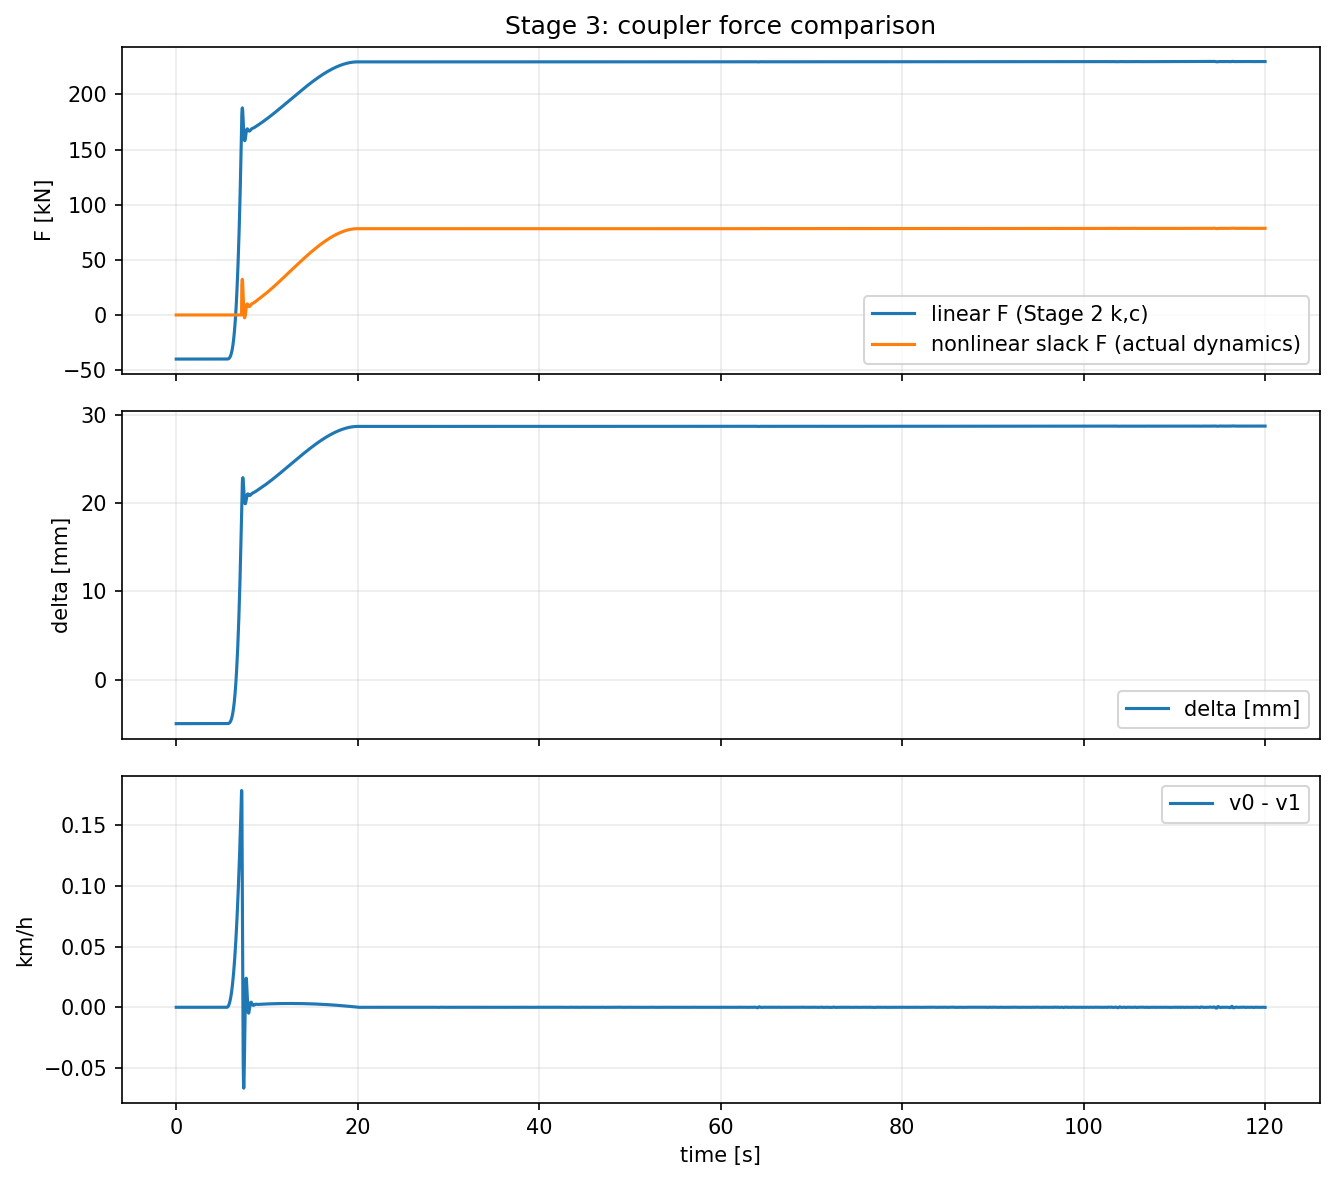
\includegraphics[width=0.92\textwidth]{../notebooks/notebook_images/ltd_stage03_slack_coupler_linear_vs_nonlinear_force_delta_speeddiff.png}
    \caption{Stage~3: comparison of linear spring-damper force (Stage~2 parameters) versus nonlinear slack coupler force along the same trajectory, with extension and relative speed.}
    \label{fig:ltd_stage03}
\end{figure}

\section{Stage 4: three bodies and sequential coupler forces}

With vehicles indexed $0,1,2$ front to rear, coupler $j\in\{0,1\}$ connects $j$ to $j+1$ and $F_j$ denotes the force on the \emph{rear} vehicle in that pair. The recursions generalise naturally:
\begin{align}
    m_0 \dot{v}_0 &= F_{\mathrm{trac}} - R_0 - G_0 - F_0, \\
    m_1 \dot{v}_1 &= -R_1 - G_1 + F_0 - F_1, \\
    m_2 \dot{v}_2 &= -R_2 - G_2 + F_1,
    \label{eq:ltd_stage4}
\end{align}
with each $F_j$ obtained from the nonlinear coupler law applied to $(\delta_j,\dot{\delta}_j)$ where $\delta_j=(x_j-x_{j+1})-L_{0,j}$. End-to-end stretch relative to nominal spacing, $(x_0-x_2)-(L_{0,0}+L_{0,1})$, summarises how the consist elongates in draft. \Cref{fig:ltd_stage04} shows speeds, both coupler forces, and stretch for a traction-only run. An optional variant applies a time-localised service-brake force on the lead only while traction continues, illustrating redistribution of draft forces (\cref{fig:ltd_stage04b}).

\begin{figure}[htbp]
    \centering
    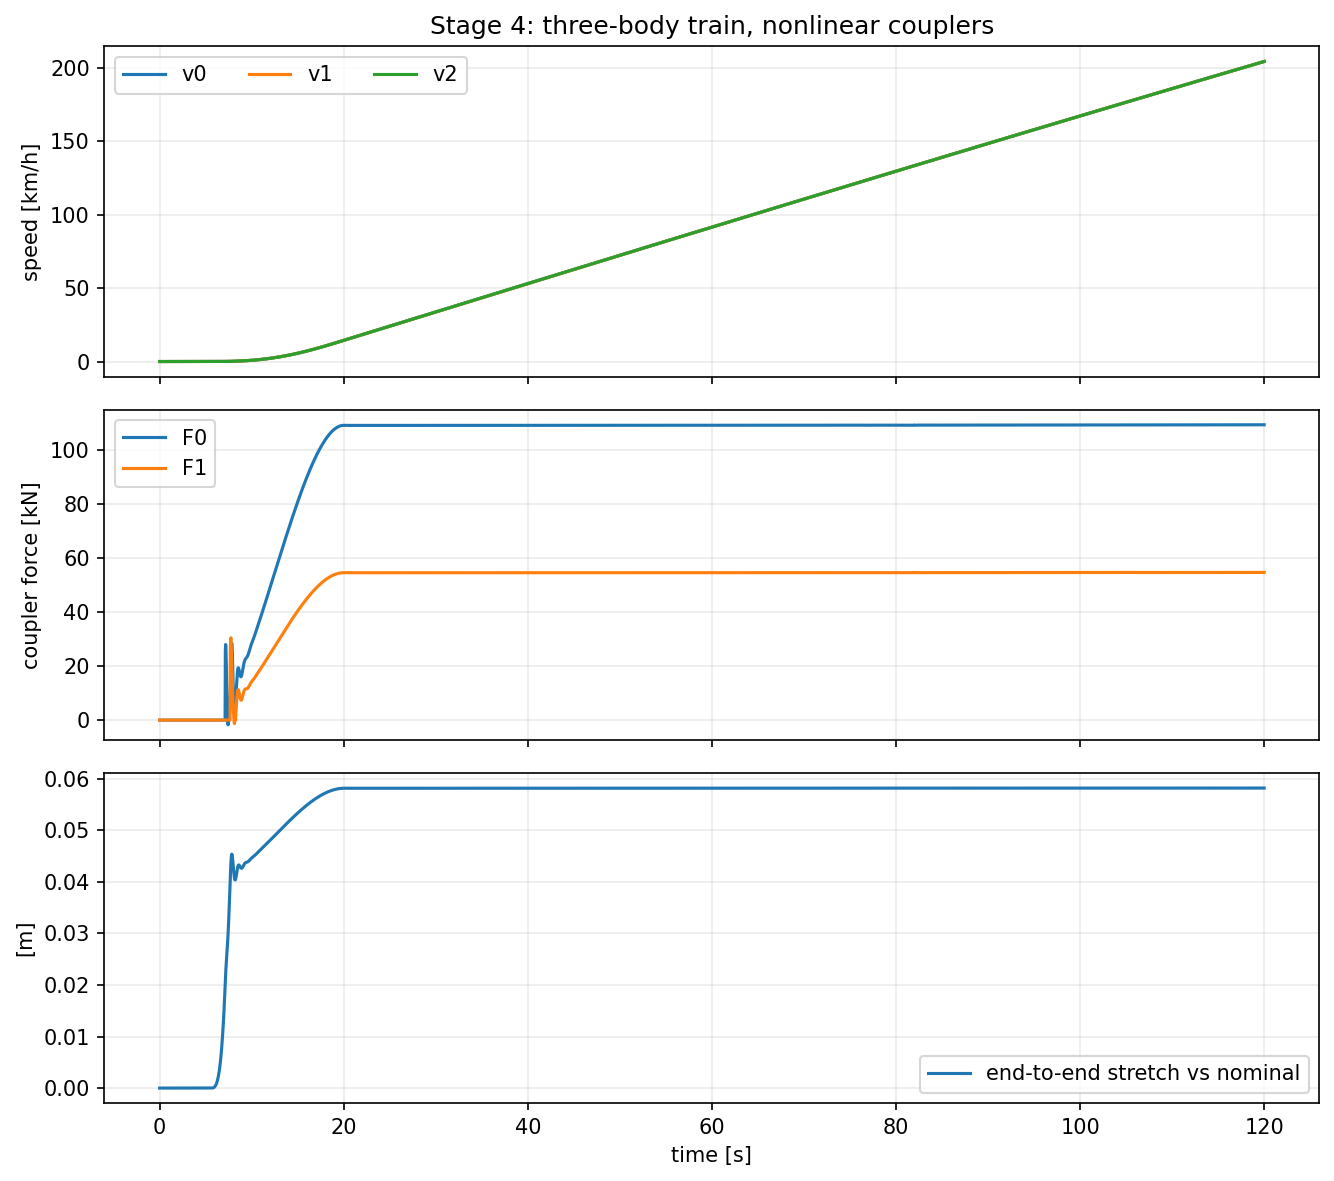
\includegraphics[width=0.92\textwidth]{../notebooks/notebook_images/ltd_stage04_three_body_speeds_coupler_forces_train_stretch.png}
    \caption{Stage~4: three-body train with nonlinear couplers. Speeds, coupler forces $F_0$ and $F_1$, and end-to-end stretch versus time.}
    \label{fig:ltd_stage04}
\end{figure}

\begin{figure}[htbp]
    \centering
    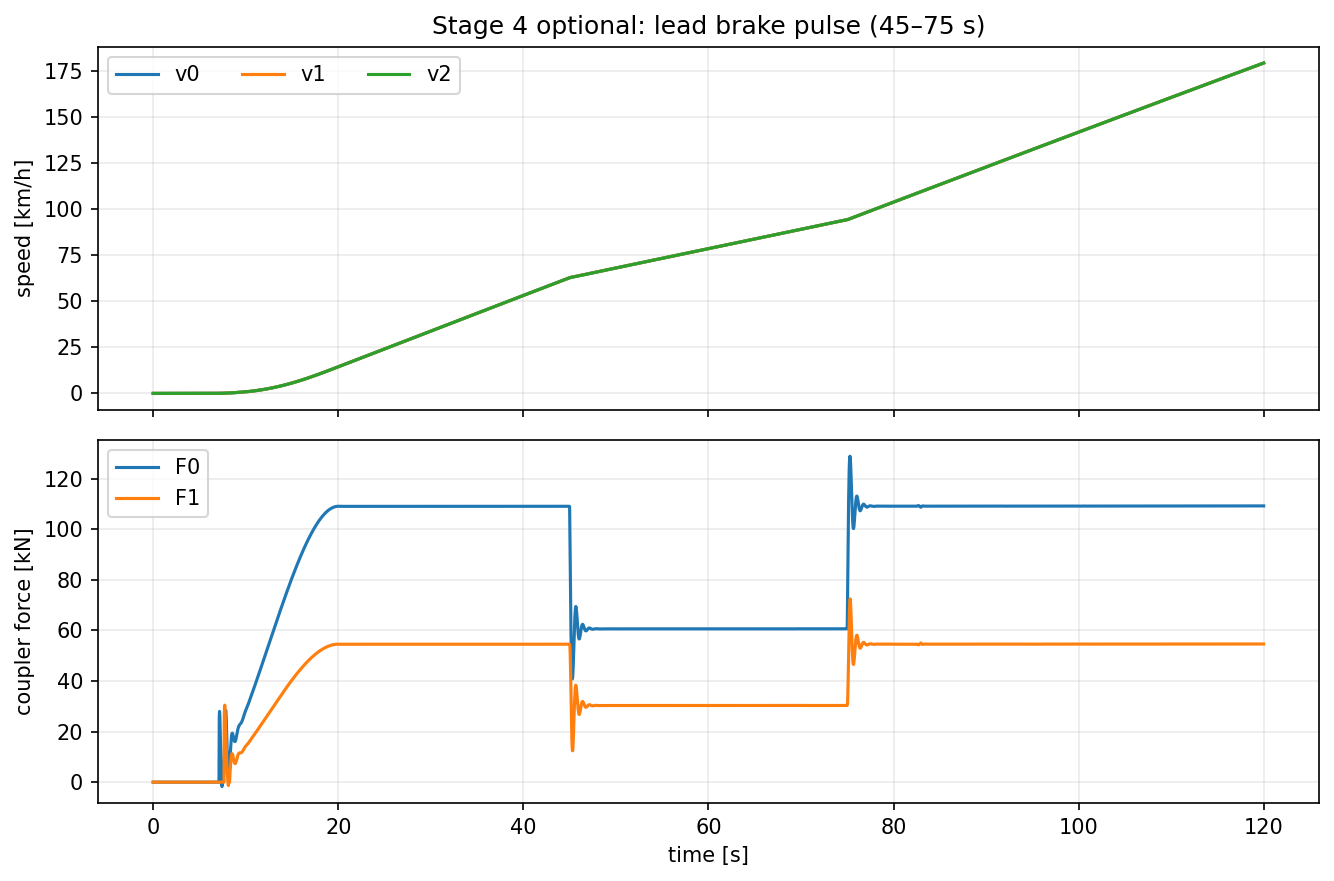
\includegraphics[width=0.92\textwidth]{../notebooks/notebook_images/ltd_stage04b_lead_brake_pulse_speeds_coupler_forces.png}
    \caption{Stage~4 optional scenario: lead-only brake pulse; speeds and coupler forces.}
    \label{fig:ltd_stage04b}
\end{figure}

\section{Stage 5: general \texorpdfstring{$N$}{N}-vehicle assembly}

The state is stacked as $\mathbf{y}=(x_0,\ldots,x_{N-1},v_0,\ldots,v_{N-1})^\top\in\mathbb{R}^{2N}$. For each coupler $j=0,\ldots,N-2$, $\delta_j$ and $\dot{\delta}_j$ are defined as in \cref{eq:ltd_delta} with vehicle $j$ ahead of $j+1$. The force $F_j$ on the rear vehicle follows the slack model with per-coupler parameters. The right-hand side for vehicle $i$ is
\begin{equation}
    m_i \dot{v}_i = F_{\mathrm{trac},i} - F_{\mathrm{brk},i} - R_i(v_i) - G_i(x_i) - C_i + F_{i-1}^{\mathrm{in}} - F_i^{\mathrm{out}},
    \label{eq:ltd_stage5}
\end{equation}
with the convention $F_{-1}^{\mathrm{in}}=F_{N-1}^{\mathrm{out}}=0$, and with traction and braking possibly zero on unpowered cars. Data structures (vehicle and coupler parameter records, and a flat route profile) group masses, Davis triples, coupler geometry, and slack/stiffness data for reuse. This is also the stage where the simulator stops being tied to a fixed train length: the same code path handles any $N$, which is what lets it later generate training data across a wide range of consist sizes rather than one fixed configuration. \Cref{fig:ltd_stage05a} plots selected speeds and coupler forces for a consist with one powered lead and identical trailing cars; \cref{fig:ltd_stage05b} shows a space-time style heatmap of all coupler forces, illustrating the monotonic decay of steady draft force from head to tail when only the lead provides traction.

\begin{figure}[htbp]
    \centering
    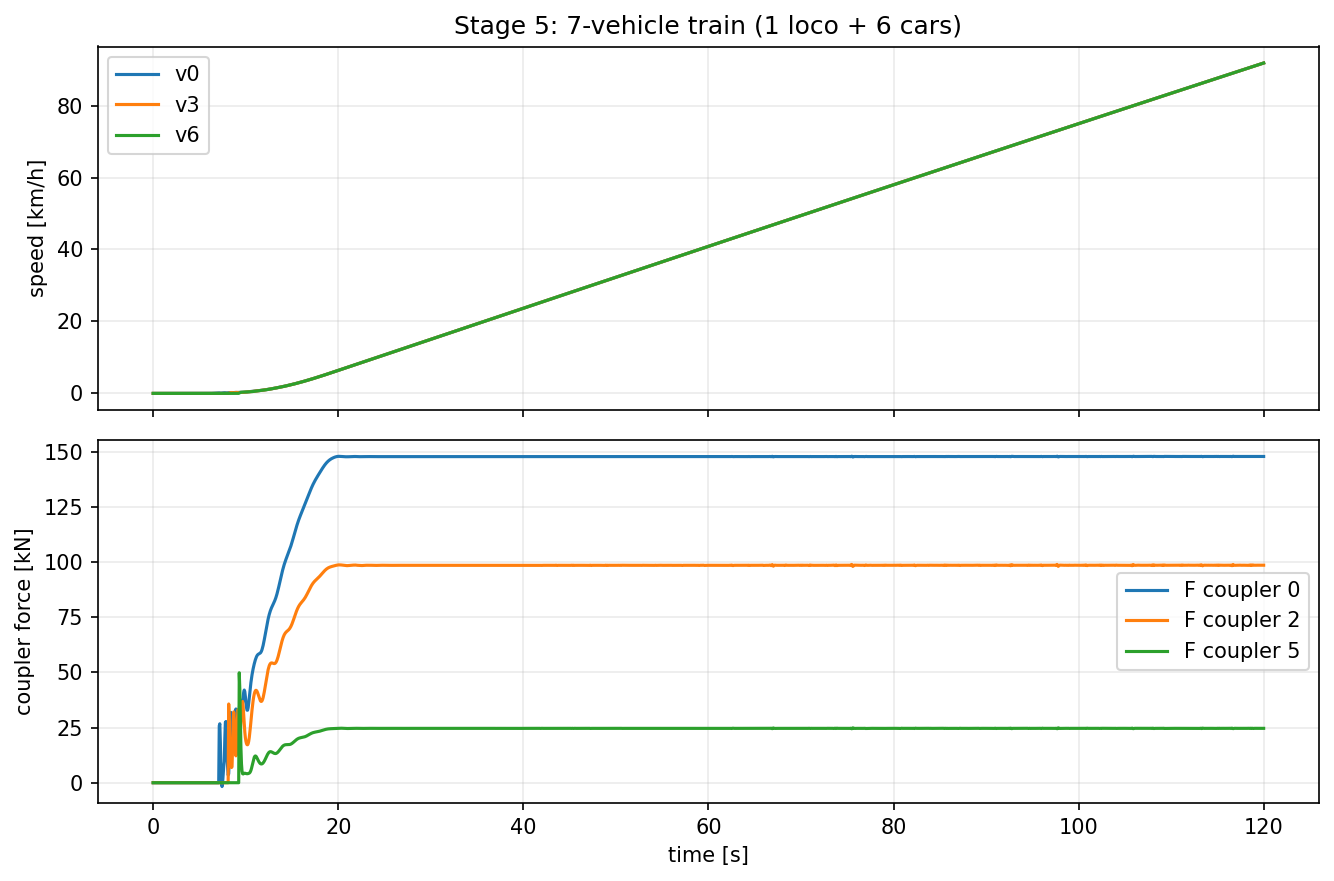
\includegraphics[width=0.92\textwidth]{../notebooks/notebook_images/ltd_stage05_N_vehicle_speeds_and_coupler_forces.png}
    \caption{Stage~5: $N$-vehicle train; selected speeds and coupler forces versus time.}
    \label{fig:ltd_stage05a}
\end{figure}

\begin{figure}[htbp]
    \centering
    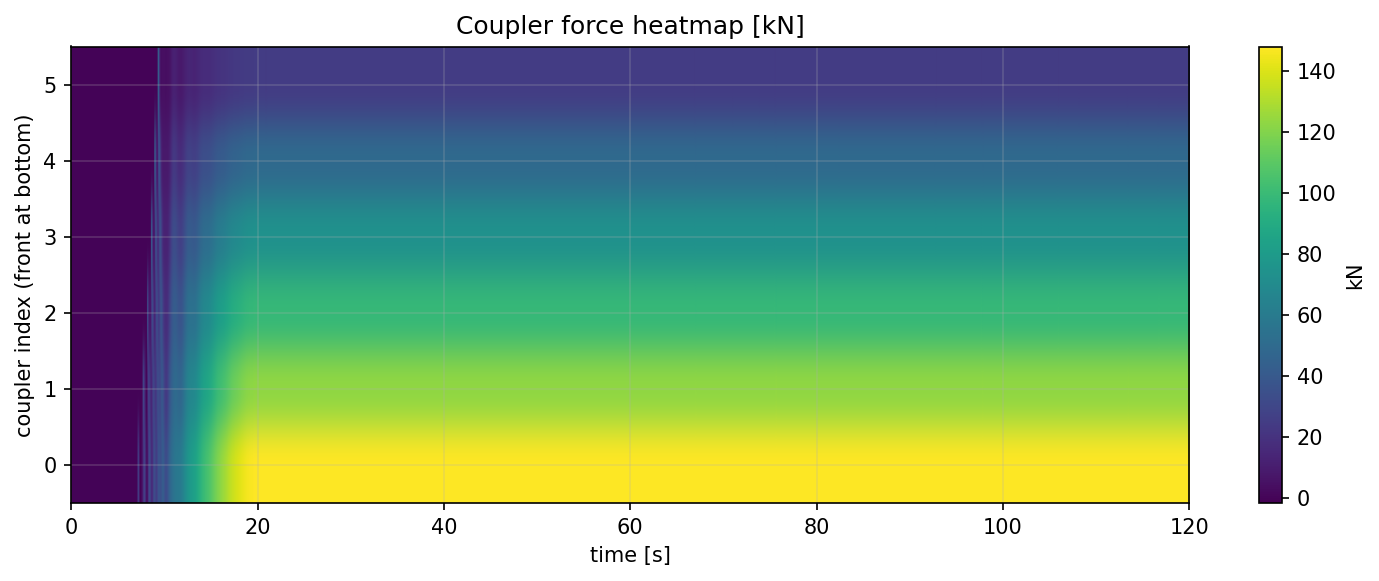
\includegraphics[width=0.92\textwidth]{../notebooks/notebook_images/ltd_stage05_N_vehicle_coupler_force_heatmap.png}
    \caption{Stage~5: coupler force heatmap (force versus time and coupler index).}
    \label{fig:ltd_stage05b}
\end{figure}

\section{Stage 6: per-vehicle grade and curvature from a route profile}

Grade and curvature are no longer evaluated at a single global $x$; each vehicle samples $\sin\theta(x_i)$ and optionally $\kappa(x_i)$ at its own position. The profile is stored as piecewise-linear nodes and interpolated (e.g.\ linearly in arc length). Then $G_i=m_i g\sin\theta(x_i)$, and \cref{eq:ltd_curvature} applies per vehicle with $m$ and $\kappa$ evaluated at that vehicle: $C_{\kappa,i}=c_{\kappa}\,m_i g\,\lambda\,|\kappa(x_i)|\,\mathrm{sgn}(v_i)$. This introduces spatial dispersion along the train: the head and tail can experience different grades simultaneously, which excites relative motion and coupler cycling even when speed traces remain nearly overlaid. \Cref{fig:ltd_stage06} shows the prescribed $\sin\theta$ along route distance in the top panel and the time evolution of lead and rear speed and selected coupler forces below; the horizontal axes of the lower panels are simulation time, not chainage, so the spatial profile should be read as a fixed map through which the train moves.

\begin{figure}[htbp]
    \centering
    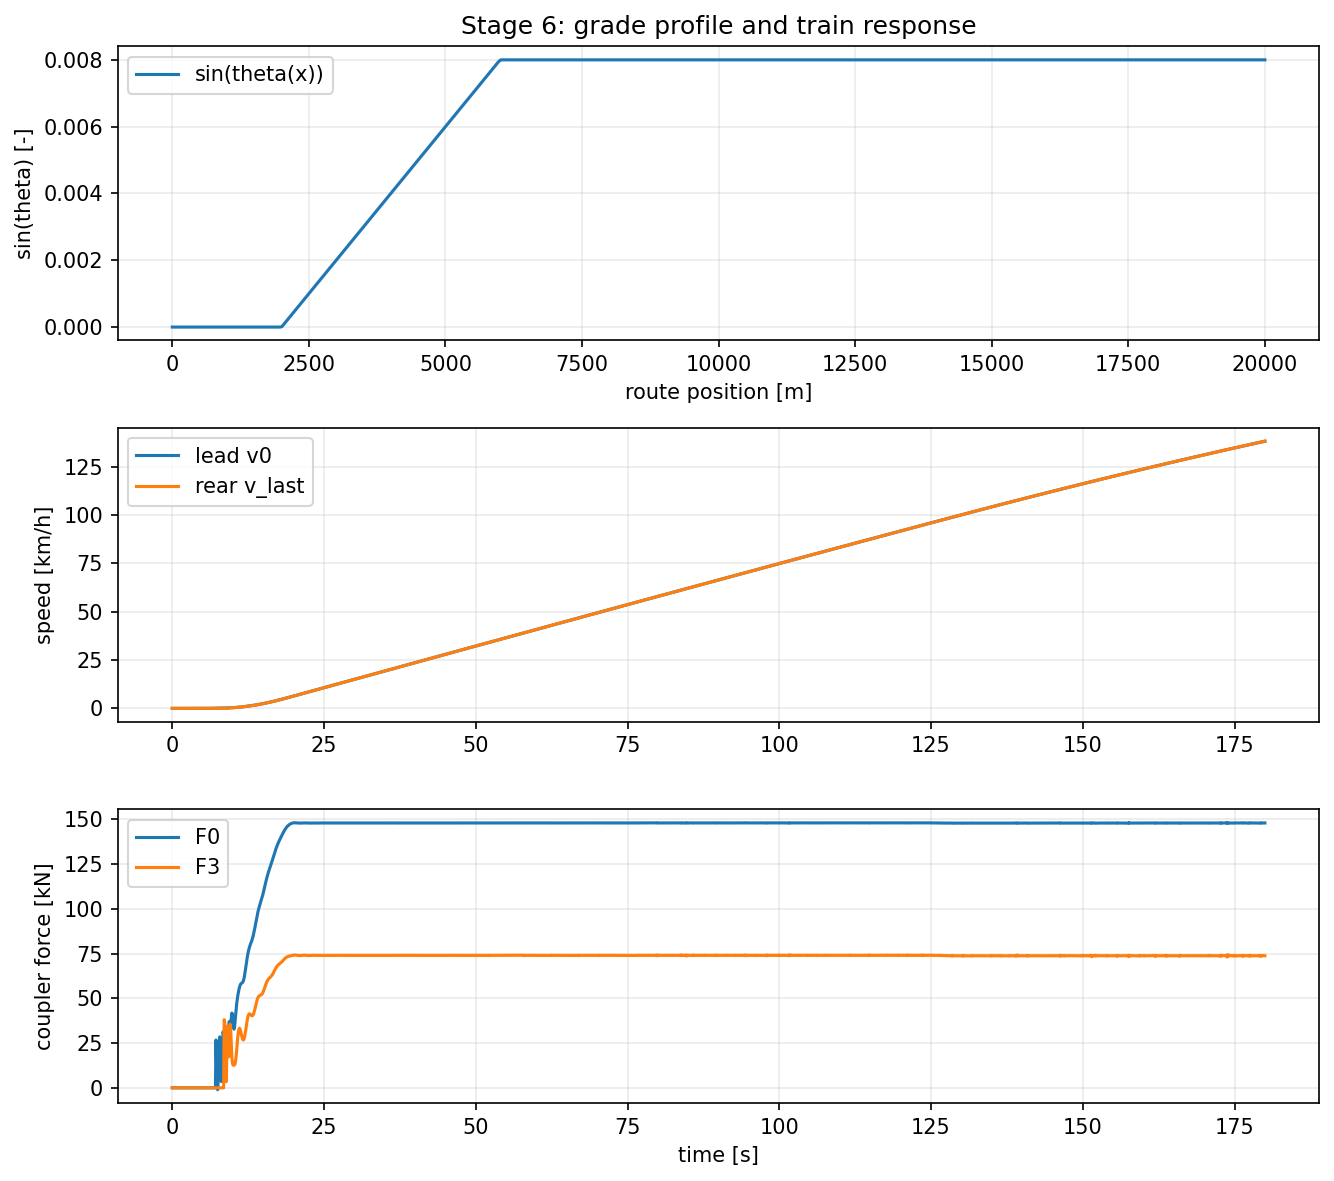
\includegraphics[width=0.92\textwidth]{../notebooks/notebook_images/ltd_stage06_grade_profile_lead_rear_speeds_coupler_forces.png}
    \caption{Stage~6: interpolated grade profile $\sin\theta$ versus route position, with lead and rear speeds and coupler forces versus simulation time.}
    \label{fig:ltd_stage06}
\end{figure}

\section{Stage 7: actuator dynamics and power-limited traction}

The state is augmented by first-order lag variables for commanded brake level $z_{\mathrm{brk},i}$ and commanded traction level $z_{\mathrm{trac},i}$ on each vehicle, driven by exogenous commands $u_{\mathrm{brk},i}(t)$ and $u_{\mathrm{trac},i}(t)$:
\begin{equation}
    \dot{z}_{\mathrm{brk},i} = \frac{u_{\mathrm{brk},i} - z_{\mathrm{brk},i}}{\tau_b}, \qquad
    \dot{z}_{\mathrm{trac},i} = \frac{u_{\mathrm{trac},i} - z_{\mathrm{trac},i}}{\tau_t}.
    \label{eq:ltd_actuator_lag}
\end{equation}
Achieved brake force is capped by a vehicle limit, $F_{\mathrm{brk},i}=\min(\max(z_{\mathrm{brk},i},0),F_{\mathrm{brk},\max,i})$, and is applied \emph{against the direction of travel} rather than in a fixed direction:
\begin{equation}
    F_{\mathrm{brk},i}^{\mathrm{applied}} = F_{\mathrm{brk},i}\,\tanh\!\left(\frac{v_i}{\varepsilon_b}\right),
    \label{eq:ltd_brake_sign}
\end{equation}
with $\varepsilon_b$ a small blend width. The $\tanh$ is preferred to $\mathrm{sgn}(v_i)$ because it keeps the right-hand side smooth through $v_i=0$, which both eases the integrator and keeps a jump in force at standstill out of the training data, where the learned step would otherwise have to reproduce it; at operating speed the factor is unity to machine precision. Without this term a vehicle braked to a standstill is accelerated in reverse without bound, since the brake would keep contributing a negative force at $v_i=0$. For powered vehicles, achieved traction is the continuous power cap
\begin{equation}
    F_{\mathrm{trac},i} = \min\!\left(\max(z_{\mathrm{trac},i},0),\,\frac{P_{\max}}{\max(|v_i|,\varepsilon)}\right),
    \label{eq:ltd_power_cap}
\end{equation}
with $P_{\max}$ an illustrative constant power ceiling and $\varepsilon$ a small speed regulariser. These substitutes replace instantaneous step forces in \cref{eq:ltd_stage5}. \Cref{fig:ltd_stage07} shows lead speed together with the lead's $z_{\mathrm{brk}}$ and $z_{\mathrm{trac}}$ for a scenario that overlaps traction command with braking command; the plotted states should not be confused with achieved $F_{\mathrm{trac},i}$ and $F_{\mathrm{brk},i}$, which also reflect \cref{eq:ltd_power_cap} and the brake saturation. This stage is what makes the control commands in \cref{ch:problem} realistic rather than instantaneous; a full driver model or anti-slip logic is outside the present scope.

\begin{figure}[htbp]
    \centering
    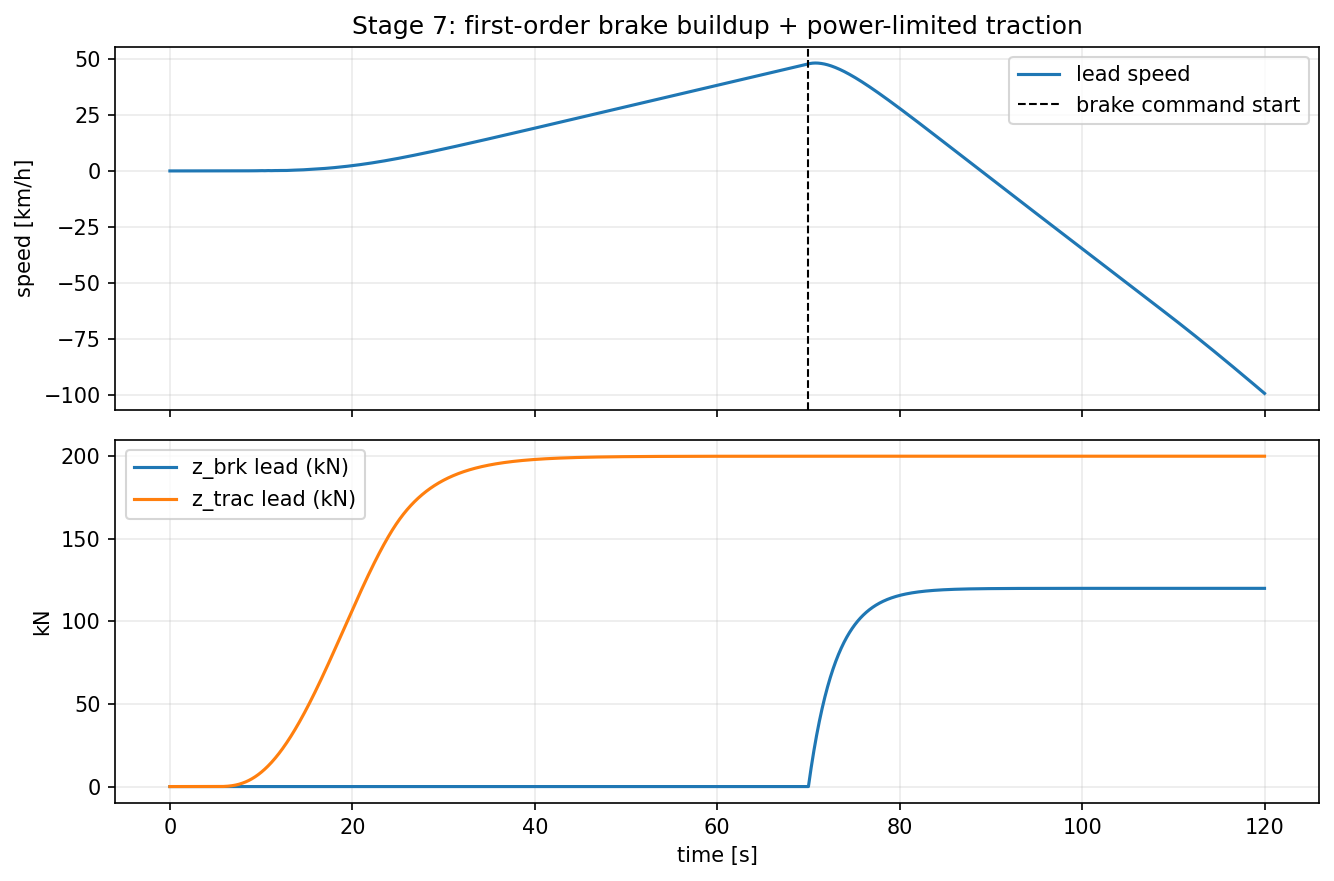
\includegraphics[width=0.92\textwidth]{../notebooks/notebook_images/ltd_stage07_brake_buildup_power_limited_traction_states.png}
    \caption{Stage~7: lead speed with brake-command onset marker; first-order lag states $z_{\mathrm{brk}}$ and $z_{\mathrm{trac}}$ on the lead versus time.}
    \label{fig:ltd_stage07}
\end{figure}

\section{Stage 8: scope relative to industrial high fidelity}

This build-up closes with a structured discussion of effects commonly associated with ``high fidelity'' in operational or research simulators: hysteretic draft gear, pneumatic brake pipe dynamics, distributed traction and adhesion limits, stochastic parameters, and calibration to field data. Those modules are not part of the reference code path summarised here; they mark the boundary between the intermediate-fidelity simulator used for learning experiments in this thesis and a fully industrial toolchain. Packaging this right-hand side as a batched GPU integrator for dataset generation is described in \cref{ch:gpu_dataset}.

\section{Chapter summary}

This chapter documented the reference simulator, built up one physical effect at a time: a single vehicle under traction and resistance, a linear coupler, a nonlinear slack coupler with asymmetric buff and draft, a general chain of $N$ vehicles, per-vehicle grade and curvature sampled from a route profile, and actuator lag with power-limited traction.
The result is a reproducible, intermediate-fidelity simulator that matches the multi-body, route-coupled structure of the problem stated in \cref{ch:problem}, and that can generate consist configurations, routes, and control plans in the volume needed to train a surrogate model.
\Cref{ch:routes} builds the real-terrain route profiles along which it is driven.
